\section{First implementation of plane wave basis: {\tt PWGrid\_01.jl}}

To describe a plane wave basis, we need to define our periodic simulation box
by specifying three lattice vectors. We also need to specify number sampling
points for each lattice vector.
We will store the lattice vector in $3\times3$ matrix.
({\color{red} add convention for lattice vectors, probably using
the same convention as PWSCF input file}).

In file {\tt PWGrid\_01.jl}, we give an implementation of plane wave basis
set, which is encapsulated in a user-defined type {\tt PWGrid}.
An instance of {\tt PWGrid} can be initialize via code like this:

\begin{juliacode}
Ns = [40, 40, 40]  # sampling points
LatVecs = 10*diagm(ones(3))  # lattice vectors for cubic system
pw = PWGrid( Ns, LatVecs )
\end{juliacode}

\subsection{Details of {\tt PWGrid}}

Let's look into details of {\tt PWGrid}.

\verb|PWGrid| is defined like this:

\begin{juliacode}
type PWGrid
  Ns::Array{Int64}
  LatVecs::Array{Float64,2}
  RecVecs::Array{Float64,2}
  Npoints::Int
  Ω::Float64
  r::Array{Float64,2}
  G::Array{Float64,2}
  G2::Array{Float64}
end
\end{juliacode}

Some explanation about these fields follow:

\begin{itemize}

\item {\tt Ns} is an integer array which defines number of sampling points
in each lattice vectors.

\item {\tt LatVecs} is $3\times3$ matrix which defines lattice vectors of
unit cell in real space.

\item {\tt RecVecs} is $3\times3$ matrix which defines lattice vectors of
unit cell in reciprocal space. It is calculated according to \eqref{eq:recvecs}.

\item {\tt Npoints} Total number of sampling points
\item {\tt Ω} Unit cell volume in real space
\item {\tt r} Real space grid points
\item {\tt G} \textbf{G}-vectors
\item {\tt G2} Magnitude of \textbf{G}-vectors

\end{itemize}

The constructor for {\tt PWGrid} is defined as follow.
\begin{juliacode}
function PWGrid( Ns::Array{Int,1}, LatVecs::Array{Float64,2} )
  Npoints = prod(Ns)
  RecVecs = 2*pi*inv(LatVecs')
  Ω = det(LatVecs)
  R,G,G2 = init_grids( Ns, LatVecs, RecVecs )
  return PWGrid( Ns, LatVecs, RecVecs, Npoints, Ω, R, G, G2 )
end
\end{juliacode}

The function {\tt init\_grid()} is defined as follow. It takes
{\tt Ns}, {\tt LatVecs}, and {\tt RecVecs} as the arguments.

\begin{juliacode}
function init_grids( Ns, LatVecs, RecVecs )
\end{juliacode}

First, grid points in real space are initialized:

\begin{juliacode}
  Npoints = prod(Ns)
  r = Array(Float64,3,Npoints)
  ip = 0
  for k in 0:Ns[3]-1
  for j in 0:Ns[2]-1
  for i in 0:Ns[1]-1
    ip = ip + 1
    r[1,ip] = LatVecs[1,1]*i/Ns[1] + LatVecs[2,1]*j/Ns[2]
              + LatVecs[3,1]*k/Ns[3]
    r[2,ip] = LatVecs[1,2]*i/Ns[1] + LatVecs[2,2]*j/Ns[2]
              + LatVecs[3,2]*k/Ns[3]
    r[3,ip] = LatVecs[1,3]*i/Ns[1] + LatVecs[2,3]*j/Ns[2]
              + LatVecs[3,3]*k/Ns[3]
  end
  end
  end
\end{juliacode}

In the next step, grid points in reciprocal space, or \textbf{G}-vectors
and also their squared values are initialized

\begin{juliacode}
  G  = Array(Float64,3,Npoints)
  G2 = Array(Float64,Npoints)
  ip    = 0
  for k in 0:Ns[3]-1
  for j in 0:Ns[2]-1
  for i in 0:Ns[1]-1
    gi = mm_to_nn( i, Ns[1] )
    gj = mm_to_nn( j, Ns[2] )
    gk = mm_to_nn( k, Ns[3] )
    ip = ip + 1
    G[1,ip] = RecVecs[1,1]*gi + RecVecs[2,1]*gj + RecVecs[3,1]*gk
    G[2,ip] = RecVecs[1,2]*gi + RecVecs[2,2]*gj + RecVecs[3,2]*gk
    G[3,ip] = RecVecs[1,3]*gi + RecVecs[2,3]*gj + RecVecs[3,3]*gk
    G2[ip] = G[1,ip]^2 + G[2,ip]^2 + G[3,ip]^2
  end
  end
  end
\end{juliacode}

The function {\tt mm\_to\_nn} defines mapping from real space to Fourier space:

\begin{juliacode}
function mm_to_nn(mm::Int,S::Int)
  if mm > S/2
    return mm - S
  else
    return mm
  end
end
\end{juliacode}

Finally, the variables \verb|r|, \verb|G|, and \verb|G2| are returned.

\begin{juliacode}
  return r,G,G2
\end{juliacode}


\subsection{Visualizing real-space grid points}

In the directory \verb|pwgrid_01|, we visualize grid points in real space
using Xcrysden program. Originally Xcrysden, is meant to visualize crystalline structure,
however, we also can use it to visualize grid points, taking periodic boundary
conditions into consideration.
This is useful to check whether grid points are generated correctly or not.

\begin{figure}
\centering
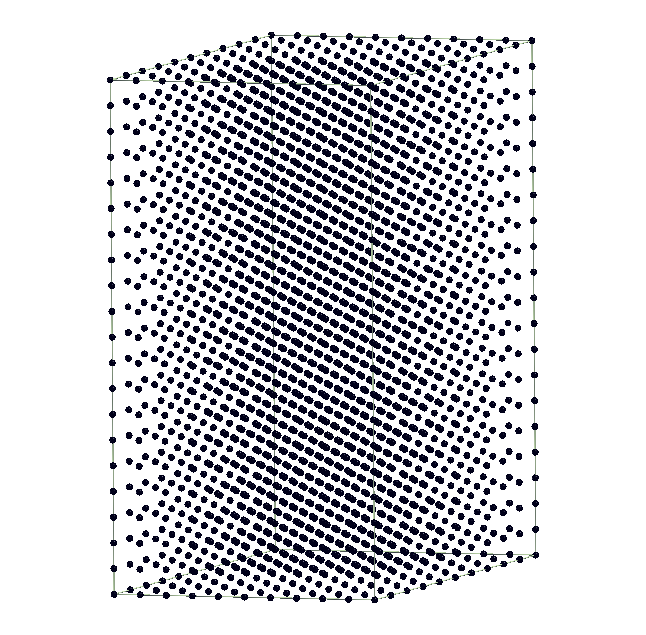
\includegraphics[scale=0.25]{images/R_grid_hexagonal.png}
\par
\end{figure}
